%!TEX root = ../main/main.tex

En esta sección, se explicará tanto la indumentaria utilizada para la implementación del código como la metodología que se empleó para ajustar la ecuación (\ref{1}) a un problema esférico. 

\subsection{Indumentaria para elaboración de código}
Para el tratamiento del código --el que ya había sido avanzado en clases del curso-- se utilizó la siguiente indumentaria para efectos del estudio del modelo MC y el transporte de partículas:

\begin{table}
	\centering
	\begin{tabular}{|c|c|c|}
		\hline 
		 INDUMENTARIA \\
		\hline
		Computador \\ \hline
		Lenguaje de programación C \\ \hline
		Bibliografía y clases teóricas del curso \\
		\hline 
	\end{tabular} 
	\caption{Tabla resumen con la indumentaria utilizada.}
\end{table} 

\subsection{Metodología de implementación}
En primera instancia, dado que, el código ya tenía un avance previo hecho en clases del curso, había que notar que el mismo estaba implementado para secciones eficaces del tipo prismáticas, vale decir, no había una simetría esférica para un estudio y análisis como el que se pedía en el enunciado del proyecto. Esto significó un punto clave para poder adecuarlo a la realidad del informe, por lo que toda la geometría tuvo que ser cambiada a simetría esférica. \\

Luego, se eligieron mediante generadores de números seudoaleatorios un punto dentro del núcleo de material fisionable con probabilidad uniforme de ocurrencia, para así, escoger un vector unitario --también con probabilidad uniforme-- que cumpliese el rol de vector director inicial de la partícula: al implementar esto dentro de un ciclo, el programa irá siempre verificando posiciones iniciales y finales de la partícula, definiendo en toda vez este vector y sumándole el camino libre medio para que la partícula experimente \emph{sampling}. En tanto, también había que definir las condiciones de paso por región: la esfera maciza constaba de cuatro regiones: un núcleo y tres cascarones, por lo que se hacía necesario comunicarle a la partícula en qué región estaba para luego establecer el análisis estadístico pedido. \\

\begin{figure}[h!]
	\label{fig:1}
	\centering
	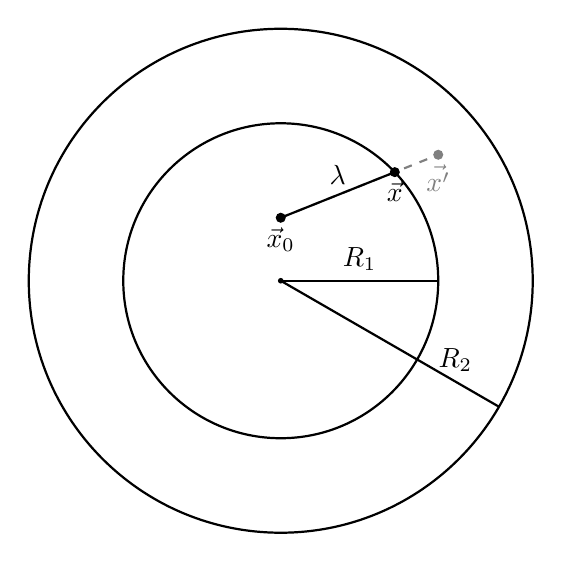
\begin{tikzpicture}[scale=.8]

		\draw[black, thick] (0,0) circle (2.5);
		\draw[black, thick] (0,0) circle (4);
		\draw[gray, thick, dashed] (0,1) -- (2.5,2);
		\filldraw[gray] (2.5,2) circle (2pt) node[anchor=north] {$\vec{x'}$};

		\filldraw[black] (1.8103,1.7241) circle (2pt) node[anchor=north] {$\vec{x}$};

		\draw[black, thick] (0,1) -- (1.8103,1.7241) node[pos=0.5, above] {$\lambda$};

		\draw[black, thick] (0,0) -- (2.5,0) node[pos=0.5, above] {$R_1$};
		\draw[black, thick] (0,0) -- (3.464,-2) node [pos=0.8, above] {$R_2$};
		\filldraw[black] (0,1) circle (2pt) node[anchor=north] {$\vec{x}_0$};
		\filldraw[black] (0,0) circle (1pt);
	\end{tikzpicture}
	\caption{Diagrama de cambio de región}
\end{figure}


La mayor dificultad en la adaptación del algoritmo radicó en calcular la distancia necesaria que debe recorrer la partícula para llegar a la frontera de la región a la cuál se quiere cambiar. Esta distancia corresponde a el valor $\lambda$ presente en la figura 1. Para encontrar este valor hay que resolver la intersección entre la recta definida por el punto inicial $\vec{x}_0$ y el vector director $\vec{u}$, con la esfera de radio $R_1$, esto es:

\begin{align}
	(x, y, z) &= (x_0, y_0, z_0) + \lambda(u, v, w) \\
	x^2 + y^2 + z^2 &= R_1^2
\end{align}

Lo que nos da una ecuación cuadrática para $\lambda \in [0, \infty)$. Esta ecuación es

\begin{equation}
	(u^2+v^2+w^2) \lambda^2 + 2(ux_0+vy_0+wz_0) \lambda + (x_0^2 + y_0^2 + z_0^2 - R_1^2) = 0
\end{equation}

Cuya solución está dada por (considerando que $(u^2+v^2+w^2) = 1$):

\begin{equation}
	\lambda = \frac{-2(ux_0+vy_0+wz_0) + \sqrt{4(ux_0+vy_0+wz_0)^2 - 4(x_0^2 + y_0^2 + z_0^2 - R_1^2)} }{2}
\end{equation}

El caso es general para cualquier cambio de región.









  